\documentclass[sigconf]{acmart}

\usepackage[utf8]{inputenc}
\usepackage{url}
\usepackage{todonotes}


% ACM Garbage
\setcopyright{none}
\begin{abstract}
As software systems grow in size and complexity, the task of manual debugging consumes more time in the development cycle, and opens up to more serious and frequent human error. To address this problem, researchers have developed systems for automated patch generation, which attempt to reduce the manual work required for diagnosing and addressing faulty code. Machine Learning models, which can leverage large amounts of information, for example from large code repositories, promise one possible set of solutions for automated patch generation. In particular, researchers have recently used sequential generative adversarial networks (GANs) successfully in text-based prediction tasks. We thus propose a model for sequential generative adversarial networks for automated patch generation (SeqGAN-APG) which divides the task of patch generation into a two-part adversarial framework which learns the distribution of sequential features in non-buggy code while also learning to generate sequential features which mimic that distribution. Our approach is novel not only in terms of its application of GANs to an untested kind of sequential data, but also in terms of the kinds of sequential features which we implement, going beyond the typical token-based approach. 
\end{abstract}
\acmConference[]{}{}{} 
\acmYear{2017}
\copyrightyear{2017}

\begin{document}

\title{SeqGAN-APG: Sequential Generative Adversarial Networks for Automatic Patch Generation}


\author{Bradley Baker}
\affiliation{%
  \institution{University of New Mexico}
  \city{Albuquerque} 
  \state{New Mexico}
}
\email{bbradt@unm.edu}
\keywords{Automatic Patch Generation, Generative Adversarial Networks, Deep Learning}

\maketitle

\section{Introduction}
\label{sec:intro}
As software systems grow in size and complexity, the task of manual debugging consumes more time in the development cycle, and opens up to more serious and frequent human error. So far in 2017, Mozilla has verified 576 newly reported bugs for the Firefox web-browser \cite{FirefoxBugdays}, a complex piece of software containing nearly 18 million lines of code \cite{FirefoxOpen}. Though many discovered bugs may only affect the system at a superficial level, some faults can expose serious security vulnerabilities, and thus require immediate attention and resolution - an often tall order in large and complex software systems. In the past decade, researchers have thus begun to turn toward automatic bug-detection and repair in an effort to address the rising difficulties of manual debugging \cite{arcuri2008automation}; however, few of the proposed methods have made use of recent advances in machine learning and artificial intelligence in order to leverage information regarding software structure, history, or other relevant data.

As machine learning has been celebrating a wide array of novel applications, many researchers have applied machine learning models to problems in software engineering and design, leveraging large repositories of code as data sets to solve various problems. For example, one popular line of research has translated solutions for movie recommender systems to help Integrated Developing Environments predict API calls while writing programs \cite{bruch2009codecomplete,asaduzzaman2014cscc,robillard2010recommendation}. Only recently, however,  researchers have started to leverage large code repositories to help in automated patch generation and other security-related problems. In this paper, we provide a contribution towards this effort in the form of a Sequential Generative Adversarial Network for Automated Patch Generation (SeqGAN-APG). Our proposed framework utilizes a discriminative model trained in an adversarial setting to learn the underlying distribution of novel sequential features extracted from buggy and non-buggy programs, while the associated generative adversarial model attempts to learn how to generate the kinds of sequential features characteristic to non-buggy code. This represents a novel approach to deep learning for patch generation, contrasting with the auto-encoder based method recently implemented in the Deepfix Patch Generation framework \cite{gupta2017deepfix}.

Though our implementation currently lacks some final details and sufficient time to learn thorough models, which will establish SeqGAN-APG as a full pipeline, our implemented discriminative and generative models do provide sequential predictions for the target distribution of non-buggy programs. In addition to the standard approach of utilizing sequences of tokens to represent program data, our model utilizes a novel application of AST-based sequential features for generating non-buggy code samples, thus taking an important step into the application of alternative sequential features which may better capture the rigid syntactical structures at work in programs. 

\section{Background}
\label{sec:background}
In this section, we present some of the background information at work in our presentation of SeqGAN-APG. 
% We first present a brief review of the problem of Automatic Patch Generation from a methods standpoint - we formalize the problem for our framework specifically in section \ref{}. We secondly present a brief discussion on different approaches to program representation for machine learning purposes. Finally, we briefly overview Generative Adversarial Networks, and specifically Generative Adversarial Networks for Sequences, since these models form the basis for the discriminative and generative tasks which fuel our framework. 

\subsection{Automated Bug Repair}
\label{sec:auto_bugrep}
We can divide the problem of automatic bug repair into a number of sub-problems: "failure detection (something wrong has happened), bug diagnosis (why this has happened), fault localization (what the root cause is), [and] repair inference (what should be done to fix the problem)" \cite{monperrus2014critical}. In addition to this taxonomy, "repair inference" can be extended to include "patch generation"\footnote{These methods often target security-related goals \cite{cui2007shieldgen,sidiroglou2005countering}} if the final product of the model is a full software patch intended to produce a concrete resolution for a bug or set of bugs within software. In the past, many researchers have approached each of these sub-problems individually (see, for example \cite{monperrus2015automatic,dallmeier2007extraction,kim2006automatic,liu2005sober,lukins2010bug}), while some frameworks attempt to address multiple problems at once, often performing both localization and repair (e.g. \cite{long2016automatic}). Historically, repair inference has perhaps most frequently been addressed using genetic programs (\cite{forrest2009genetic,arcuri2008novel,le2012genprog,le2013automatic,weimer2010automatic,kim2013automatic}), although a number of other approaches utilize other methods such as solving problems in Satisfiability Modulo Theory  \cite{demarco2014automatic,xuan2017nopol}, or semantic analysis \cite{nguyen2013semfix}. Most recently, some state of the art methods have taken some first steps into data mining \cite{le2016history} and even some basic probabilistic methods \cite{long2016automatic}; however, the problem of bug repair via patch generation has been largely untouched by machine-learning, and thus deserves further exploration.

Our approach, insofar as it incorporates a discriminative model in association with a generative model for creating patches sits at the intersection of failure detection and patch generation, with additional work remaining in fault localization to apply generated patches to buggy code.

\subsection{Program Representations for Machine Learning}
\label{sec:programreb}
 In cases where researchers use program repositories as data for machine learning models, the problem presents itself - how do we represent a program so that a model can successfully leverage the information included therein? %Most generally we can model a program $P$ as a data-tensor $P \in \mathcal{X}^n$  with $n$ features, where we select a choice of features based on a particular choice of features extracted from $P$.
 
Following work in natural language processing, one popular set of approaches encodes program features in terms of sequences and subsequences of tokens present in the program. A simple bag-of-words approach, for example, indicates the presence of particular tokens in a program, without including any sequential information, while a more sophisticated approached might encode the presence of $n$-length grams, i.e. repeated patterns of tokens. Researchers have used these and other highly sparse, token-based features to successfully encode programs for analysis purposes. For additional discussion of text representations in machine learning see \cite{allahyari2017text,ramya2017feature}.
 
Another popular representation of program information is the program's abstract syntax tree (AST). The AST of a program provides a graph-based representation of relationships between particular syntactical objects in the program, thus capturing more detailed information about a program's underlying structure, such as relationships between variable types, the scope of certain statements and structures, etc.

%A third kind of program representation is the logical-formulae representation, a popular tool of theoretic computer science which has appeared in some automated applications, but which has seen relatively little application in machine learning. This lack of application is most likely due to a lack of thorough automated tools for converting programs to logical representations, with the automation of invariant selection being one established difficult sub-problem in this well-explored field \cite{waldinger1969prow, rodriguez2007generating}.

Finally, programs as a data objects often contain a number of additional features not included in text data. One could very well include program creation or modification timestamps, input-output evaluations, runtime information, or other program data as features of $P$. While a large body of work in machine-learning focuses on text-representations alone, the frontier of feature engineering and selection for program data remains wide open for both sequential and non-sequential feature types. 

\subsection{Generative Adversarial Networks}
\label{sec:gans}
The underlying model which motivates our proposal of SeqGAN-APG is a Generative Adversarial Network (GAN) \cite{goodfellow2014gan}. A generative adversarial network is a \textit{joint} learning framework involving two deep neural networks, which trains both models in a joint setting to perform two different, but related tasks: one model, the generative model, attempts to emulate the distribution of a given target data set; the second, discriminative model, attempts to estimate the probability that a given sample came from a training data set rather than from $D$. The generative model, attempts to act as an adversary for the discriminator, using reinforcement learning techniques to attempt to learn how to 'fool' the discriminator, thus hopefully increasing the robustness of the discriminator as well as the ability of the generator to replicate the target distribution.

Researchers have applied GANs to a number of interesting generative tasks, mostly centered around image generation (e.g. \cite{denton2015imagegan}) and other real-valued data. It is only very recently that researchers have begun to explore the application of generative adversarial networks to discrete, sequential information, such as text \cite{zhang2017adversarial, press2017langgan}. The SeqGAN \cite{yu2017seqgan} model in particular has illustrated that utilizing Recurrent Neural Networks along with some tweaks to gradient computations for the generative task can provide robust sequence predictions. The idea behind SeqGAN-APG is to use this sequential generative adversarial network to generate sequential samples which mimic the distribution of non-buggy programs, while also training a discriminator which is attempting to distinguish between distributions of buggy and non-buggy programs. %In the following section, we discuss a formalization of this problem, and describe our methodology for implementing it on the CodeFlaws data set of buggy and non-buggy programs.

\section{Methodology}
\label{sec:methods}
In this section we describe the underlying methodology used to formulate, build, and evaluate SeqGAN-APG. %We first formalize the problem of automatic patch generation in terms of the dual tasks of bug discrimination and patch generation, approaching the latter task in a more general fashion than previous models which restrict the problem to token prediction. We then discuss the methods used to process data for testing two kinds of sequential representations of programs: sequences of tokens and AST representations. Next, we present the entire SeqGAN-APG framework, and discuss the details of its implementation. Finally, we present our methodology for evaluating SeqGAN-APG in comparison to several baseline methods for automated patch generation, which follows previous methods in terms of evaluating successful patches, but which is novel in terms of the scope of comparisons to other models. 

\subsection{Model Formulation}
\label{sec:model}
The problem of automatic patch generation bears closest resemblance to structured sequence prediction, insofar as the underlying generator strives to predict the correct sequence of tokens which will replace a buggy snippet of code. As mentioned before, we want to train a Sequential Generative Adversarial Network for Automatic Patch Generation (SeqGAN-APG), so we split the task of automatic patch generation into 1) buggy vs. non-buggy discrimination, and 2) sequential feature generation. 

\textbf{Buggy/Non-Buggy Discrimination}

Let $P$ be a program or snippet represented by a given set of features $\{F_i\}$ such as ordered sequences of tokens, input-output specifications, runtime information, etc. Additionally, associate a binary label $L$ to each program indicating whether the program does ($L == 1$) or does not ($L == 0$) contain a bug. The basic task of automatic patch generation posits a model $M$ which best emulates the map	$M: \{P_{L == 1}\} \rightarrow \{P_{L == 0}\}$.

The majority of previous approaches to automatic patch generation select a "best" candidate patch from a restricted search-space generated from restricted transformations on the features of $P$. The model in \cite{long2016automatic}, for example, learns a probabilistic ranking over the features of successfully patched data in order to rank an automatically generated search space for $P$, created by permuting specific features of $P$, such as the structure of the Abstract Syntax Tree, or sequences of tokens.

While restricting models to predictions on restricted search-spaces can help to retain certain structures on candidate patches, it does so at the expense of excluding possibly successful candidates not available in the search space. Our approach, in contrast, strives to learn the underlying distribution of features in buggy and non-buggy programs, and to use this discriminatory power to drive an underlying generative process for generating a non-buggy program given a set of features for a buggy program.  Thus, our approach generalizes from learning a particular map on a known or assumed set of distributions to learning a model which learns estimates of the underlying distributions in order to predict whether or not a given program sample represents a buggy or non-buggy problem. This first task is thus allocated to the \textit{discriminative} part of the Sequential Generative Adversarial Network.

\textbf{Sequential Feature Generation}

We choose to adopt the intuition that many program features include sequential information which may prove important in characterizing the distribution of buggy and non-buggy programs, and to treat the problem of patch generation as a kind of structured sequence generation. This idea follows the example of Deepfix's sequence-to-sequence patch generation \cite{gupta2017deepfix}, which posits a model for translating sequences of buggy tokens to sequences of non-buggy tokens using the Seq2Seq deep auto-encoder \cite{luong2015seq2seq}. Though the underlying network structure of SeqGAN-APG is fundamentally different than Deepfix, we approach patch generation in fundamentally the same way. Given a buggy program or snippet $P$, with a set of sequential features $X_1, ..., X_n$, and a set of non-sequential features $\{F_i\}$, our model attempts to predict the best sequence of target features $Y_1, ..., Y_n$ such that the resulting patched program best resembles the learned distribution of non-buggy programs. Doing this in a joint setting allows the generative model to generate these sequential features (such as sequences of tokens or AST-nodes) to best create non-buggy programs or snippets after being given a set of buggy programs as input. Additionally, the sequential nature of the features mean that if a fault is localized, the trained generative model should be able to start at a location prior to the localized fault and generate a set of sequential features, such as correct tokens, which represent a fix to that localized issue.

%Following precedent in automated natural language translation, the sequence of tokens provided in a given snippet of code make one obvious  choice of sequential features for a given program. For example, \cite{gupta2017deepfix} utilize this representation, encoding each token in the sequence along with a fixed line number, so that the predicted sequence maps one-to-one with tokens in the provided buggy program. This representation, however, is not the only kind available, and may not be the best choice for predicting program patches, insofar as the structure of program language syntax is often more rigid than natural language.  

\textbf{Model Implementation Details}

Due to space constraints we have assembled the parameters and architectural details used to build the SeqGAN-AST network in appendix \ref{app:model_params}. 

% As mentioned above, Abstract Syntax Trees are one popular representation for capturing the underlying structure of a program which are not based off token presence alone, but which also capture structure such as statement scope, sequences containing particular types, or more complex characteristics such as object polymorphism. After some processing, Abstract Syntax Trees can also be represented as sequences, and can perhaps be used in lieu of, or in addition to sequences of tokens to aid in automatic patch generation. In principal, we believe that sequential and non-sequential features outside of the tokens themselves could and should be used to aid in the task of patch prediction, and that restricting patch prediction to token prediction alone is not necessary - until a more principled analysis in done which analyses the valuation of particular kinds of sequential features in programs, we follow the more general format of learning the underlying distribution of features for non-buggy programs to predict a particularly useful set of sequential features (tokens, AST-nodes, or some other feature). Figure \ref{} diagrams this general prediction task, and in the following section, we discuss the steps we take to test multiple kinds of program features, both sequential and non-sequential, that can be used in this general task of structured sequence prediction.

\subsection{Data Processing}
\label{sec:data_proc}
Our chosen data set for evaluation is the CodeFlaws data set \cite{tan2017codeflaws}, a recently released set of labeled, buggy and non-buggy programs written in the C programming language. Each file in the CodeFlaws data has a label of either buggy or non-buggy, includes a set of nine input-output evaluations, and matches with a dual file of the opposite label written for the same program functionality.  Additionally, each buggy file contains a label identifying the particular kind of bug under the codeflaws proposed taxonomy of bugs \cite{tan2017codeflaws}, which means we could possibly extend learning the binary discriminative task of buggy and non-buggy programs to learn the distributions of features characterizing certain \textit{kinds} of bugs.

Prior to analysis, we remove include statements and comments from each file, assuming that bugs are not located in the usage of particular headers, and aren't influenced by information in comments. This also restricts the vocabulary to only statements which are parsed on compilation, and which do not require the linking of external libraries or header files. We then format the C files so that the contents of each file are all located on a single line, and assemble positive and negative files into separate data sets, where each row in the data set represents one file, i.e. one instance of a bug. Thus, we do not perform any kind of bug localization, treating the entire program as a positive or negative instance of the bug, rather than extracting snippets or labeling lines separately. 

This initial approach to data representation requires the length of input and output sequences to be quite long (between 100 and 400 tokens on average), which makes the generation task difficult. This lack of bug localization means we cannot currently associate generated samples with particular fault locations. This major shortcoming short-circuits the final step of the patching pipeline, and represents a major point of remaining work.

\textbf{Token-Sequence Representation}

After assembling C files into the separated data sets as described above, we first generate a data set which encodes programs as sequences of tokens. In each line of the positive and negative files, we first convert all recognized C operators into unique tokens, using the intuition that each operator has a semantic meaning in a similar fashion to C keywords. We then use a pre-built vocabulary of C keywords and operators (based on \cite{cKeywords}) to convert tokens into unique hashes, and then extend this vocabulary to hash variable names, constants, literals, and other unique values which appear throughout the program repositories. The resulting sequence of unique hashes, along with the vocabulary for the entire repository, constitute the tokenized data set. %A full example of the tokenization processing pipeline is illustrated in figure \ref{fig:tokn_meth} in appendix \ref{}.

\textbf{AST-Node-Sequence Representation}

In addition to the tokenized representation of program data, we also assemble a data set based on parsing the Abstract Syntax Trees for each program. For each program, we run the Python C-AST Parser \cite{bendersky2017pycparser} in order to generate the associated AST. Once we've generated each AST, we then flatten the AST into an ordered sequence of AST nodes. To do this, we recursively parse through the entire AST in a depth first fashion, adding each encountered node to the sequence and re-encoding edges to children as sparse features in the node itself. We then use the Sklearn vectorizor \cite{pedregosa2011scikit} to convert each node to a set of hashes which encode the unique, nominal features of the given, such as the node's type, its links to other nodes in the AST, or its particular syntactical attributes such as expression or data type. The resulting data set is a tensor with a number of data instances equal to the number of files, with each instance encoding a sequence of feature vectors corresponding to the node located at the given point in the sequence.

This approach to AST-to-Sequence conversion is inspired by the approach outlined in \cite{rabinovich2017ast}, with the essential difference being that we do not convert nodes to program actions prior to parsing. % An example of this parsing technique for a small tree is given in figure \ref{fig:ast_meth}. 

\subsection{Evaluation Protocol + Baselines}
\label{sec:evaluation}
Due to the lack of a mechanism for bug localization and patch insertion, to evaluate the success of the generative model, we qualitatively compare the kinds of sequences generated from each model respectively. We compare SeqGAN with an implementation of the Seq2Seq deep learning library \cite{luong2015seq2seq}, which is the underlying network at work in the Deepfix Automatic Patch Generation suite \cite{gupta2017deepfix}. We evaluated both SeqGAN-APG and Seq2Seq on both Tokenized and AST-based data sets, and used the same preprocessing steps for both models, except for vocabulary hashing, which Seq2Seq handles internally. We have outlined the detailed parameters for running the Seq2Seq baseline have been outlined in appendix \ref{app:model_params}. In the future, we would like to implement the full Deepfix Automatic Patch Generation suite \cite{gupta2017deepfix}, in addition to other smaller suites used for automatic patch generation; however, since we have not currently resolved the localization sub-problem for our model, this comparison is currently not possible.

In addition to the Generator Baselines, we also wanted to compare the discriminative model with a suite of text classifiers implemented from the sklearn library \cite{pedregosa2011scikit}. We implemented Logistic Regression without normalization and with Elastic Net Regularization, Ridge Regression, a Linear Support Vector Machine with and without feature selection, a simple perceptron classifier, a linear passive-aggressive classifier, bernoulli and multinomial naive-bayes classifiers, a k-nearest-neighbors classifier, a nearest centroid classifier, and a random forest classifier. We performed 10-fold cross validation on all models, and record the accuracy for the binary classification task. We did not perform any hyper-parameter searches for the models, with the chosen hyper-parameters for each model are specified in appendix \ref{app:model_params}. We evaluated the suite of classifiers first on the hashed tokenized text data, and then subsequently on the hashed AST sequences. Unfortunately, due to unresolved issues in the SeqGAN library, and lack of time to invent patches for the software, it was not possible to also output accuracy for the SeqGAN model. Nonetheless, the results indicate differences between the two data processing methodologies, and remain interesting for future analysis. Regardless, without sufficient time to train the networks, or run hyperparameters, it is not likely the more complex models would compare well with the simpler models which we could implement and evaluate within a shorter time-frame.

All tests were run in a 64-bit Ubuntu 17.04 environment with 8 GB of RAM and an Intel(R) i7-4790 core clocked at 3.60GHz. SeqGAN-APG and Seq2Seq were trained using CUDA on an Nvidia GeForce GTX 980 Ti GPU with 6 GB of memory. 

\section{Results and Discussion}
\label{sec:results}
In this section, we present the initial results for SeqGAN, with the hope of comparing with the various baselines discussed in the previous section. % We first present the results comparing the discriminative model with a set of text classification baselines trained on both tokenized and AST-based data sets.

\textbf{How does SeqGAN perform in the discriminative task?}
Figure \ref{fig:disc_acc} compares the accuracy measure for a suite of classifiers tested on both tokenized and AST data sets. All classifiers perform better when utilizing the AST-based data. Unfortunately implementation issues in the SeqAST library, which does not by default support accuracy evaluation, prevented direct comparison with the discriminator at this time.  
\begin{figure}
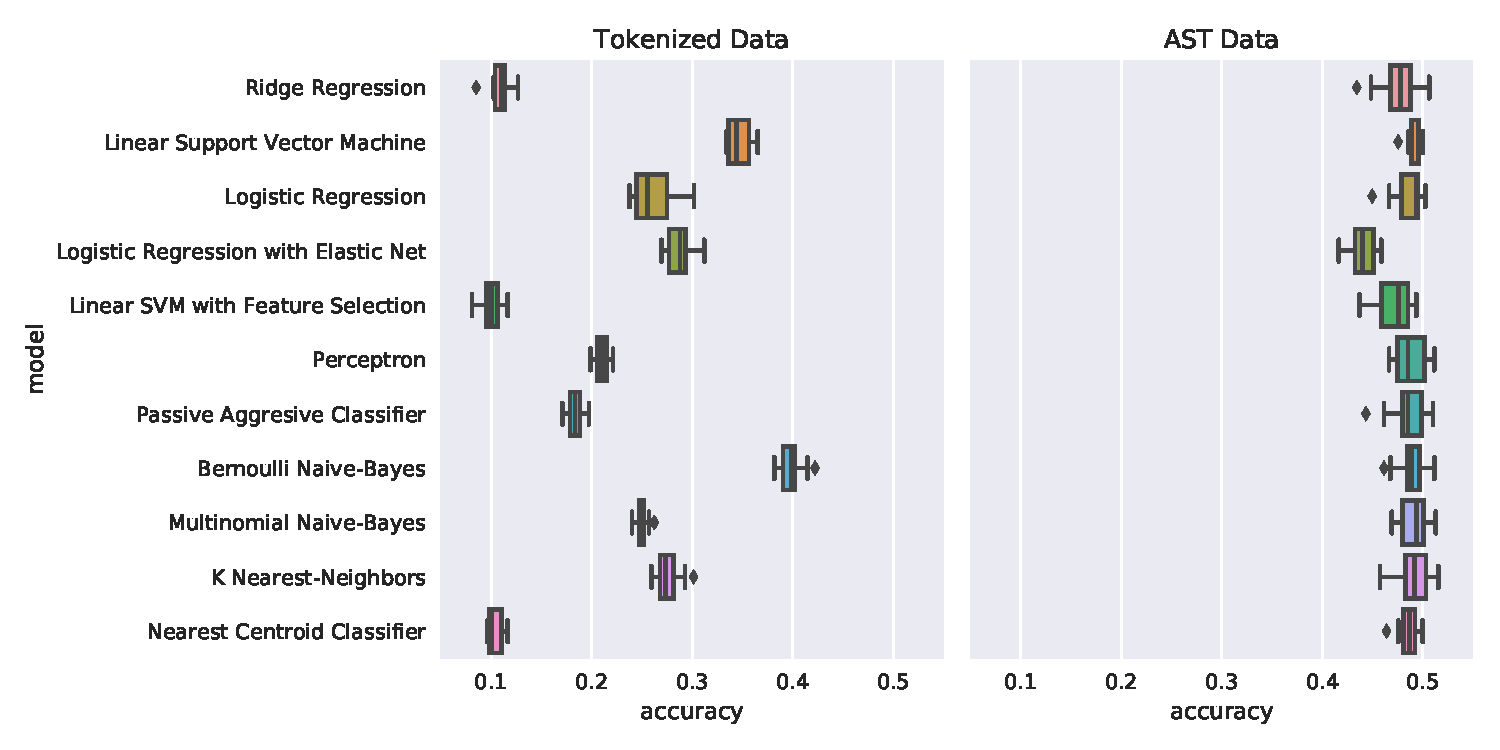
\includegraphics[width=\columnwidth]{all_clfs}
\caption{Comparison of Discrimination Accuracy on Different Data Processing Methodologies}
\label{fig:disc_acc}
\end{figure}

\textbf{What kinds of sequences do the generative models output?}

The localization issue is not the only obstacle preventing the output of currently viable patches for both generators: both deep networks require significant training time (on the order of days), as well as robust parameter tuning in order to generate viable patches, or even just viable sequences. Thus, the complexity of the models is itself a barrier to generating robust output after a short training timeframe (only 1000 or 2000 iterations, for example, is not sufficient), which is a common characteristic of most deep-learning frameworks. Access to more robust machines with more GPUs, in addition to a longer timeframe is required to generate the sequences in a more robust ways. Both models, after 1000-2000 iterations, only output sequences of operators. Thus, though the full pipelines do 'work', desirable results would require a longer time-frame.

\section{Conclusion}
\label{sec:conclusion}
In this paper, we proposed a novel Sequential Generative Adversarial Network approach to Automated Patch Generation (SeqGAN). In contrast to recent approaches in automated patch-generation, our approach utilizes an adversarial setting to learn how sequential features characterize buggy and non-buggy programs, and then use these features to build sequences of features which represent non-buggy. 

In addition to the standard representation of programs as sequences of tokens, we implemented a novel approach to model the sequential features of a program's AST nodes. Current results indicate that AST-based features help simple sequence-based classifiers to better predict whether a given program is buggy or non-buggy. Future work will also implement these features on the fully-trained, optimized generative models.

Beyond insufficient time and infrastructure to fully train and optimize the more complex models, the major missing piece of our framework is a principled strategy for localizing bugs to particular snippets of code in a fashion which would reduce the input and output sequence length, and which would aid in actually applying candidate patches to buggy code. To address this, we would adopt a similar strategy as it utilized in the DeepFix framework \cite{gupta2017deepfix}.

Altogether our framework represents an important first step toward the exploration both of utilizing different sophisticated models with different kinds of features for addressing the problem of automated patch generation. More room remains to attempt different network configurations, and to compare against various other baselines; however, the framework in its primal form is there, requiring only further polishing and few missing pieces before we can apply it in full, generative form.

\clearpage
\appendix

%\section{Data Processing Examples}
%\label{app:data_proc_ex}
%\begin{figure}[h]
%\label{fig:tokn_meth}
%\missingfigure{Token Processing Example}
%\end{figure}

%\begin{figure}[h]
%\label{fig:ast_meth}
%\missingfigure{AST Processing Example}
%\end{figure}


\section{Model Parameters}
\label{app:model_params}
In this appendix we provide the hyperparameters used to test the SeqGAN-APG model, as well as the various baselines which we implemented for comparison. If a parameter is not specified, it means the parameter was not specifically configured using the implemented API.

\subsection{Generative Models}

\textbf{SeqGAN}
Table \ref{tab:seqgan_params} outlines the parameters for the SeqGAN network utilized in SeqGAN-APG. 
\begin{table*}[ht]
	\begin{tabular}{|l|l|l|}
    \hline\textbf{Network Part} & \textbf{Parameter} & \textbf{value}\\\hline
	Generator & Embedding Dimension & 32 \\
    Generator & Hidden Dimension & 32 \\
    Generator & Sequence Length & 100 \\
    Generator & Number of Generated Samples & 500\\
	Discriminator & Embedding Dimension & 64 \\
    Discriminator & Filter Sizes & 1 - 20 \\
    Discriminator & Num Filters & 100 - 200 \\
    Discriminator & Dropout Keep Probability & 0.75 \\
    Discriminator & L2 Regularizer $\lambda$ & 0.2 \\
    Both & Batch Size & 64\\
    Both & Pre-Training Epochs & 10 \\
    Both & Training Epochs & 50 \\
	\end{tabular}
    \caption{Baseline Parameters for Discrimination Task}
	\label{tab:seqgan_params}
\end{table*}

\textbf{Seq2Seq} 
In order to assure results prior to submission, we utilized a "small" configuration of Seq2Seq with 128 units in each attention cell. In the encoding layer, we used a 0.8 input keep probability and a 1.0 output keep probability in the RNN. In the decoding layer we used a 0.8 input keep probability and a 1.0 output keep probability. We used the Adam optimizer for back-propogation, with an $\epsilon$ tolerance of $8e^{-7}$ and a learning rate of 0.0001. We capped the max sequence length at 100. See \cite{luong2015seq2seq} for more details on parameter configuration for Seq2Seq.

\subsection{Discriminative Baselines}
Table \ref{tab:dbline_params} summarizes the parameters used for the sklearn v. 0.1.2 implementation of various classifiers. 

\begin{table*}[ht]
	\begin{tabular}{|l|l|l|l|l|l|l|}
    \hline\textbf{Model} & \textbf{Maximum Iterations} & \textbf{Learning Rate} & \textbf{Tolerance} & \textbf{Number Neighbors} & \textbf{Number Estimators} & \textbf{NB-$\alpha$}\\\hline
    Ridge Regression &   &   & $1e^{-2}$ &   &   &  \\\hline
    Linear SVM &   &   & $1e^{-3}$ &   &   &  \\\hline
    Linear SVM L1-Features &   &   & $1e^{-3}$ &   &   &  \\\hline
    Linear SVM L2-Features &   &   & $1e^{-3}$ &   &   &  \\\hline
    Logistic Regression & 1000 & $1e^{-4}$ &   &   &   &  \\\hline
    Logistic Regression (EN) & 1000 & $1e^{-4}$ &   &   &   &  \\\hline
    Perceptron & 10000 &   &   &   &   &  \\\hline
    Passive Aggressive & 1000 &   &   &   &   &  \\\hline
    K-Nearest-Neighbors &   &   &   & 10 &   &  \\\hline
    Nearest Centroids &   &   &   &   &   &  \\\hline
    Random Forest &   &   &   &   & 1000 &  \\\hline
    Multinomial Naive Bayes &   &   &   &   &   & 0.01\\\hline
    Bernoulli Naive Bayes &   &   &   &   &   & 0.01\\\hline
    \end{tabular}
    \caption{Baseline Parameters for Discrimination Task}
	\label{tab:dbline_params}
\end{table*}

%\section{Additional Results}
%\label{app:additional_res}
%\textbf{How well do the models converge?}

%Figure \ref{fig:gen_loss} compares the convergence rate for SeqGAN and Seq2Seq on the tokenized and AST data sets. Under the current implementation, Seq2Seq converges much more reliably than SeqGAN, with SeqGAN actually diverging after a number of iterations, likely due to a lack of hyper-parameter tuning.

%\begin{figure}
%\label{fig:gen_loss}
%\missingfigure{Loss Comparison of generative models}
%\end{figure}
\bibliographystyle{acm}
\bibliography{project_proposal.baker}


\end{document}
